% Appendix: Ethics, Security and Generative AI documentation
% Add after \appendix in main.tex, e.g.:
% % Appendix: Ethics, Security and Generative AI documentation
% Add after \appendix in main.tex, e.g.:
% % Appendix: Ethics, Security and Generative AI documentation
% Add after \appendix in main.tex, e.g.:
% % Appendix: Ethics, Security and Generative AI documentation
% Add after \appendix in main.tex, e.g.:
% \input{app_ethics_security_ai}
%
% Image files are expected to exist in the Images/ folder exactly as named below.

\chapter{Ethics and Security Documentation}
\label{app:ethics-security}

This appendix records the ethics, research-practice and information-security documentation supporting the study. The experimental work was conducted on research models and benchmark identity-document imagery rather than against live identity-verification services. The adversarial methods were used to evaluate the robustness of detection and localisation outputs within the defined research setting, not to demonstrate an operational verification bypass. The relevant University ethics confirmation and required training evidence are reproduced below.

\section{Ethics Approval}
\label{sec:app-ethics-approval}

The project was submitted through the University ethics process. Figure~\ref{fig:ethics-approval} reproduces the ethics approval or confirmation issued for the study.

\begin{figure}[H]
    \centering
    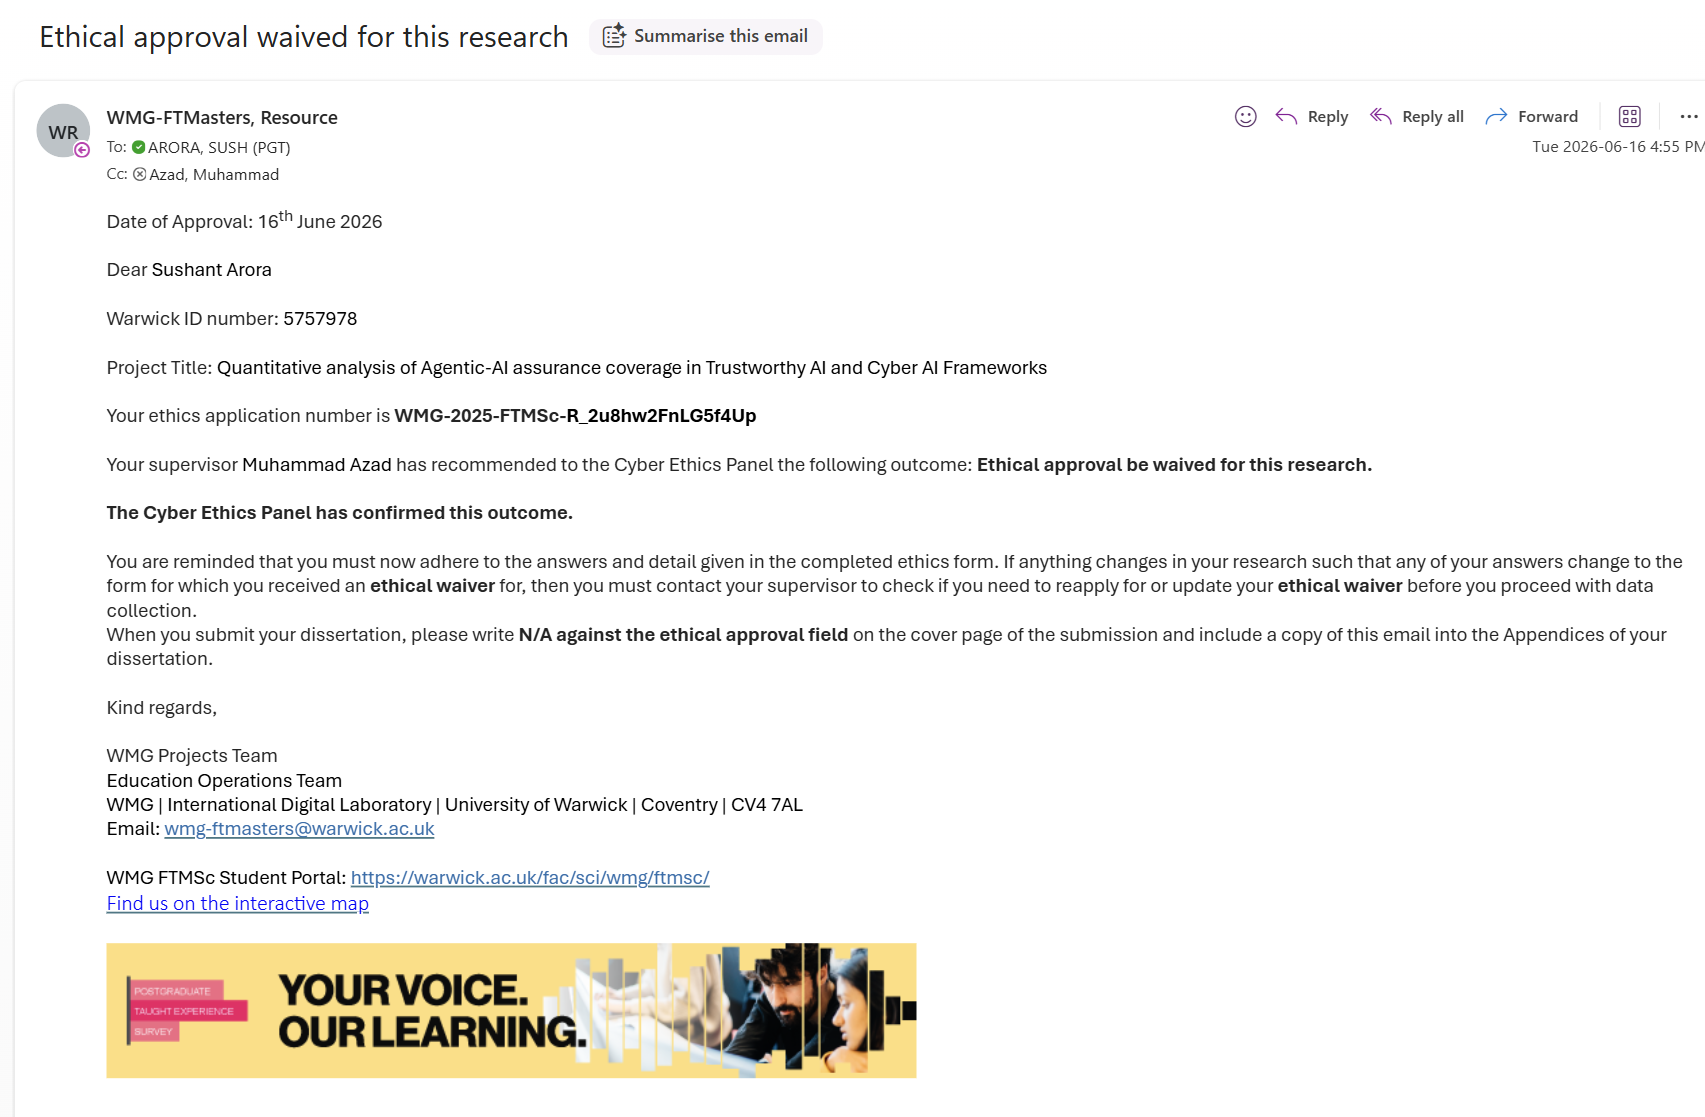
\includegraphics[
        width=0.95\textwidth,
        height=0.72\textheight,
        keepaspectratio
    ]{Images/Ethical_approval.png}
    \caption{Ethics approval or confirmation for the research project.}
    \label{fig:ethics-approval}
\end{figure}

\clearpage
\section{WMG Student Ethics Training}
\label{sec:app-ethics-training}

The WMG Student Ethics Training was completed as part of the research-governance requirements for the project. Figure~\ref{fig:ethics-training} shows the completion evidence.

\begin{figure}[H]
    \centering
    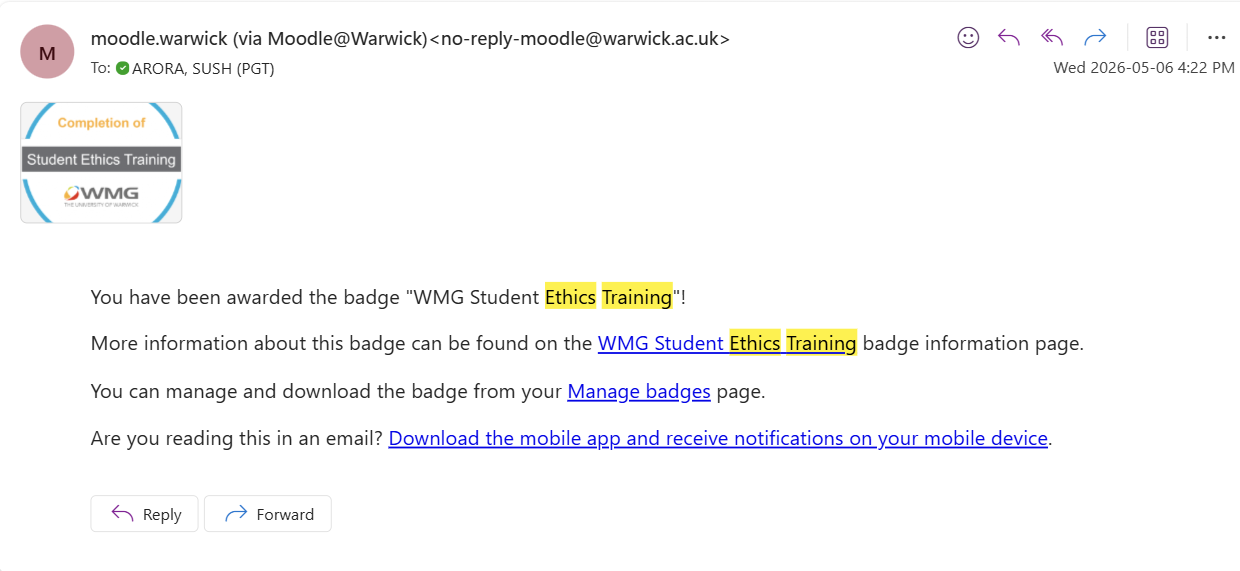
\includegraphics[
        width=0.96\textwidth,
        height=0.28\textheight,
        keepaspectratio
    ]{Images/Ethics_training.png}
    \caption{WMG Student Ethics Training completion evidence.}
    \label{fig:ethics-training}
\end{figure}

\section{Information Security Smart}
\label{sec:app-information-security}

The Information Security Smart course was completed to support appropriate handling of research data, code and computing resources. Figure~\ref{fig:information-security-smart} shows the completion evidence.

\begin{figure}[H]
    \centering
    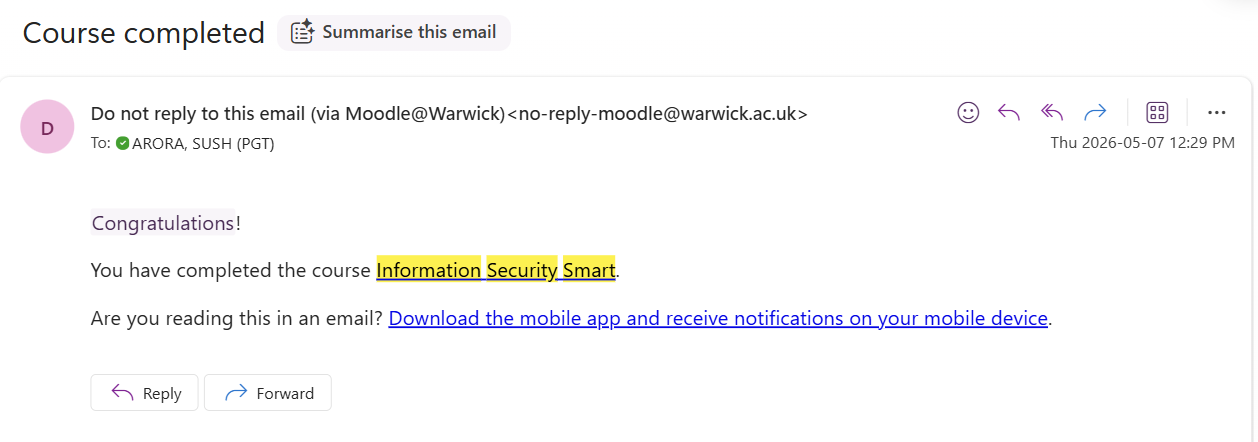
\includegraphics[
        width=0.96\textwidth,
        height=0.28\textheight,
        keepaspectratio
    ]{Images/Information_security_smart.png}
    \caption{Information Security Smart course completion evidence.}
    \label{fig:information-security-smart}
\end{figure}

\clearpage
\section{Responsible Research Practice}
\label{sec:app-responsible-research}

The Responsible Research Practice course was completed as part of the research training supporting this dissertation. Figure~\ref{fig:responsible-research-practice} reproduces the completion evidence.

\begin{figure}[H]
    \centering
    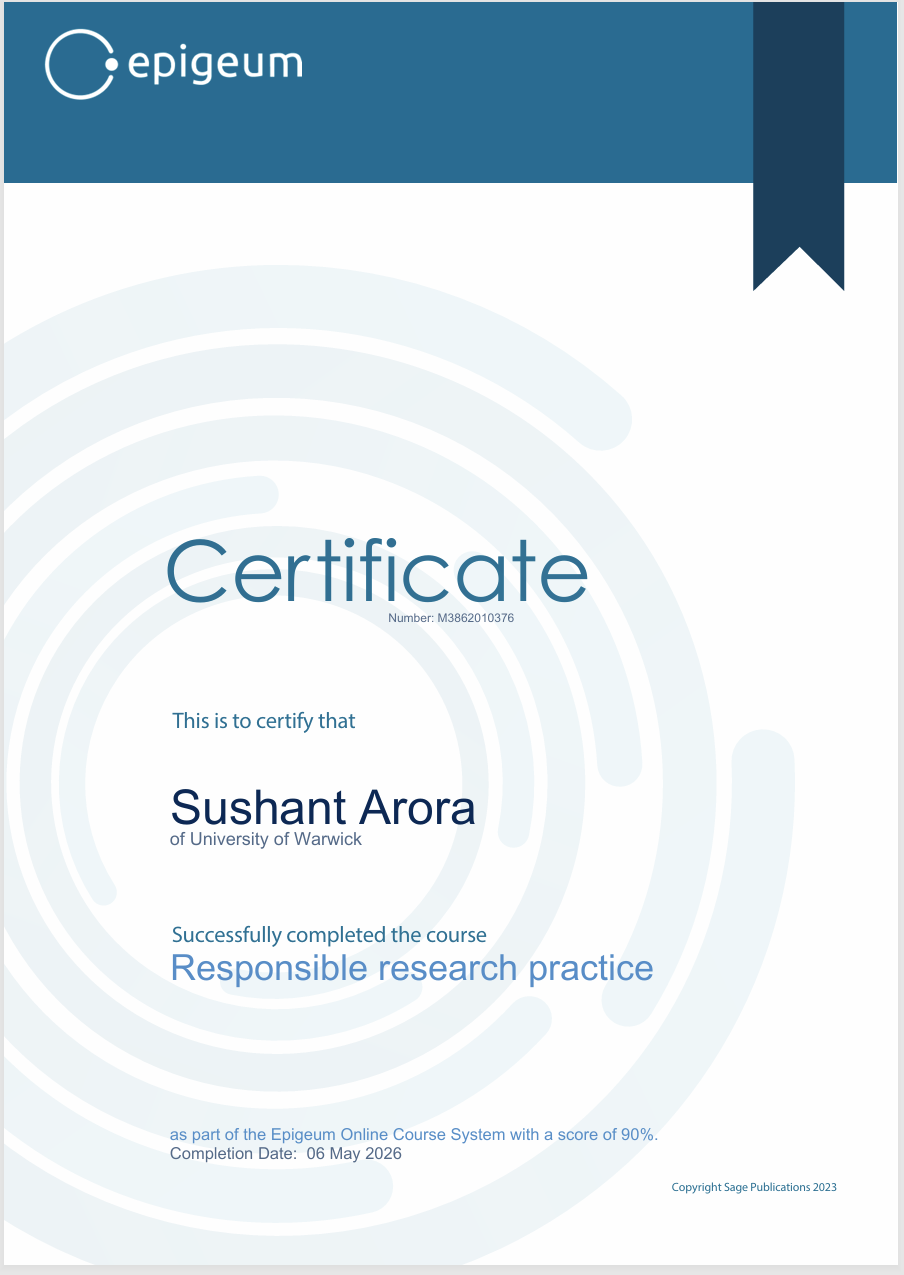
\includegraphics[
        width=0.78\textwidth,
        height=0.68\textheight,
        keepaspectratio
    ]{Images/Responsible_research_practice.png}
    \caption{Responsible Research Practice completion evidence.}
    \label{fig:responsible-research-practice}
\end{figure}

\clearpage
\section{Irresponsible Research Practice}
\label{sec:app-irresponsible-research}

The Irresponsible Research Practice course was also completed as part of the research training supporting this dissertation. Figure~\ref{fig:irresponsible-research-practice} reproduces the completion evidence.

\begin{figure}[H]
    \centering
    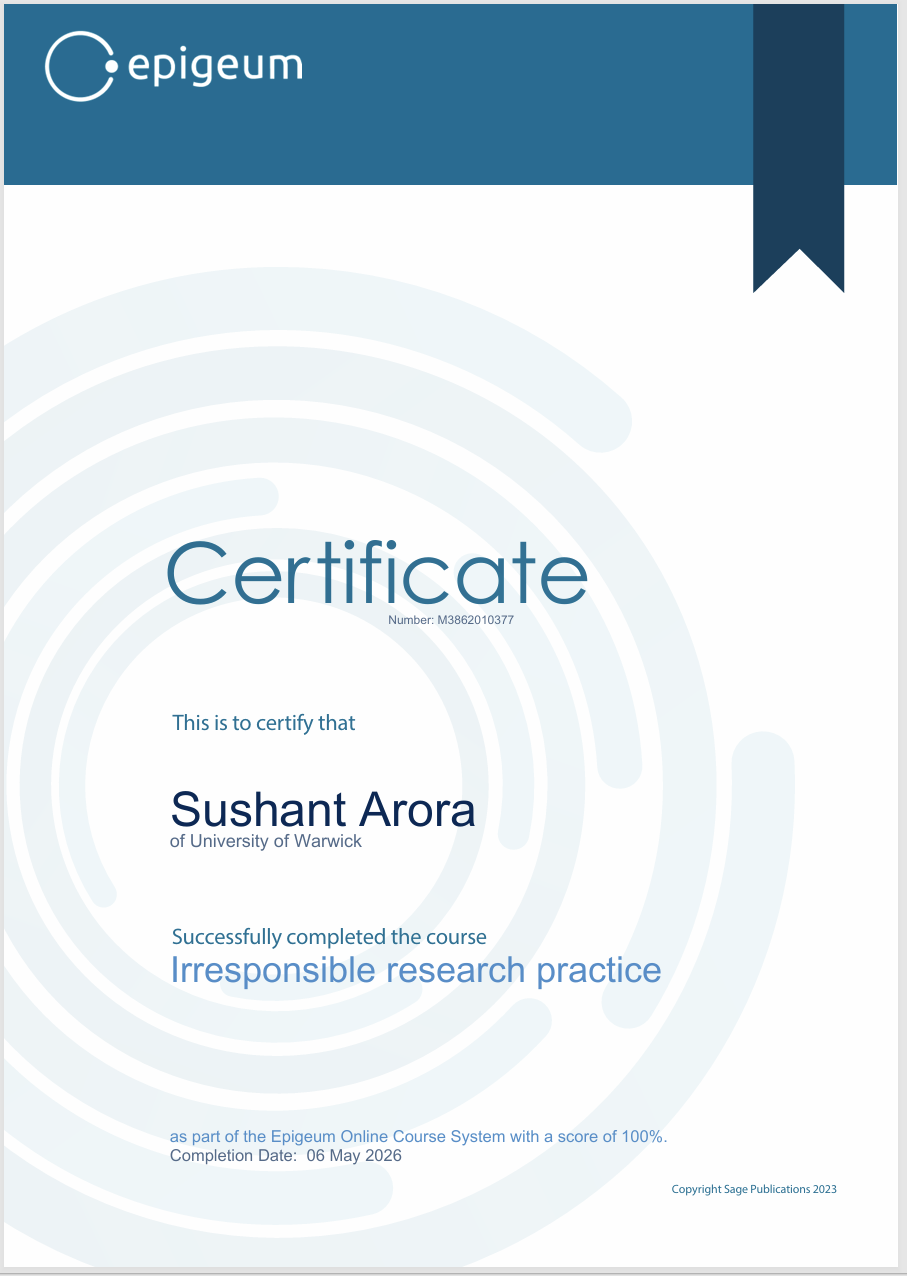
\includegraphics[
        width=0.78\textwidth,
        height=0.68\textheight,
        keepaspectratio
    ]{Images/Irresponsible_research_practice.png}
    \caption{Irresponsible Research Practice completion evidence.}
    \label{fig:irresponsible-research-practice}
\end{figure}


\chapter{Generative AI Declaration}
\label{app:generative-ai}

\section{Statement of Disclosure}
\label{sec:app-generative-ai-disclosure}

Generative Artificial Intelligence (GenAI) tools were used as supportive tools during the planning, development and preparation of this dissertation. Their use did not replace independent academic judgement, validation of experimental outputs or responsibility for the submitted work.

GenAI was used to generate boilerplate code and generic implementation patterns. This material was not adopted unchanged: it was reviewed, tested and modified for the specific data structures, model pipelines, evaluation logic and reproducibility requirements of the project. GenAI was also used for idea refinement and as a planning aid when developing the experimental execution strategy. This included considering experiment ordering, parallel execution, checkpointing and other practical choices intended to make efficient use of the available GPU hours.

Where GenAI-generated suggestions concerned code or experimental procedures, they were incorporated only after review and validation within the project workflow. GenAI outputs were not treated as experimental evidence and did not substitute for measured model outputs. The methodological decisions, verification of results, interpretation of findings and final submitted content remain the author's responsibility.

%
% Image files are expected to exist in the Images/ folder exactly as named below.

\chapter{Ethics and Security Documentation}
\label{app:ethics-security}

This appendix records the ethics, research-practice and information-security documentation supporting the study. The experimental work was conducted on research models and benchmark identity-document imagery rather than against live identity-verification services. The adversarial methods were used to evaluate the robustness of detection and localisation outputs within the defined research setting, not to demonstrate an operational verification bypass. The relevant University ethics confirmation and required training evidence are reproduced below.

\section{Ethics Approval}
\label{sec:app-ethics-approval}

The project was submitted through the University ethics process. Figure~\ref{fig:ethics-approval} reproduces the ethics approval or confirmation issued for the study.

\begin{figure}[H]
    \centering
    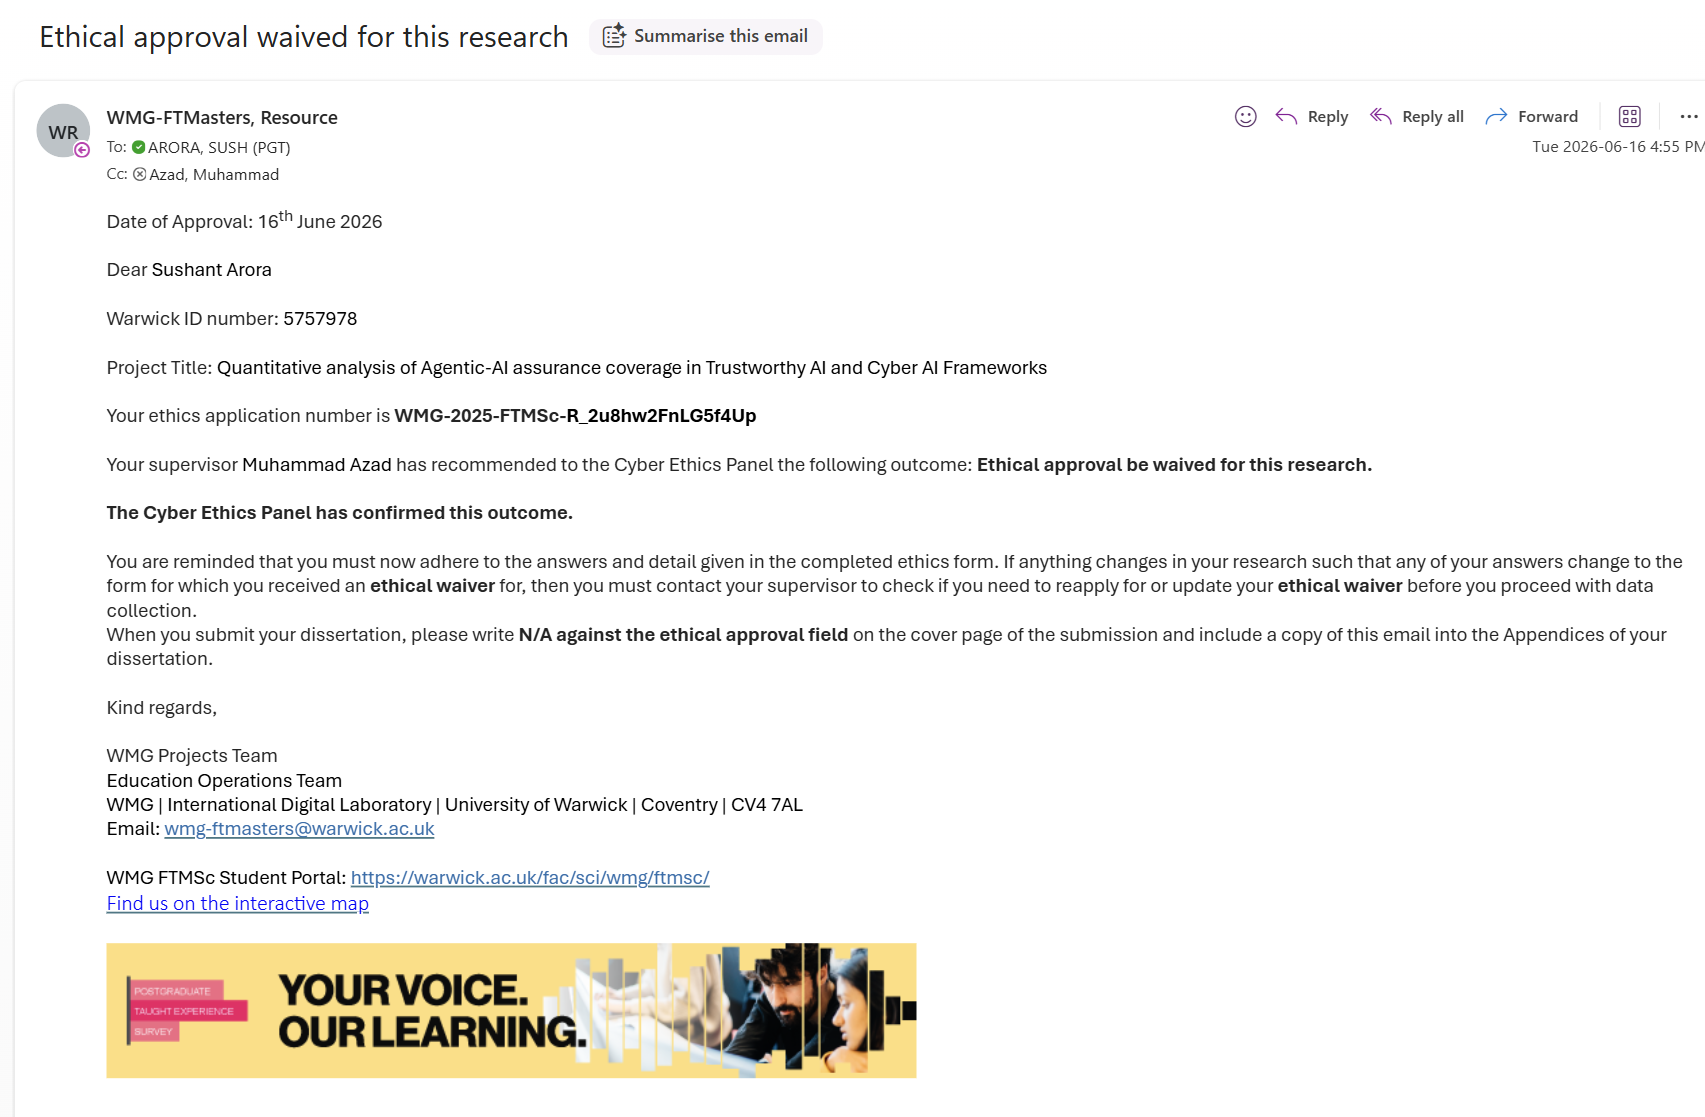
\includegraphics[
        width=0.95\textwidth,
        height=0.72\textheight,
        keepaspectratio
    ]{Images/Ethical_approval.png}
    \caption{Ethics approval or confirmation for the research project.}
    \label{fig:ethics-approval}
\end{figure}

\clearpage
\section{WMG Student Ethics Training}
\label{sec:app-ethics-training}

The WMG Student Ethics Training was completed as part of the research-governance requirements for the project. Figure~\ref{fig:ethics-training} shows the completion evidence.

\begin{figure}[H]
    \centering
    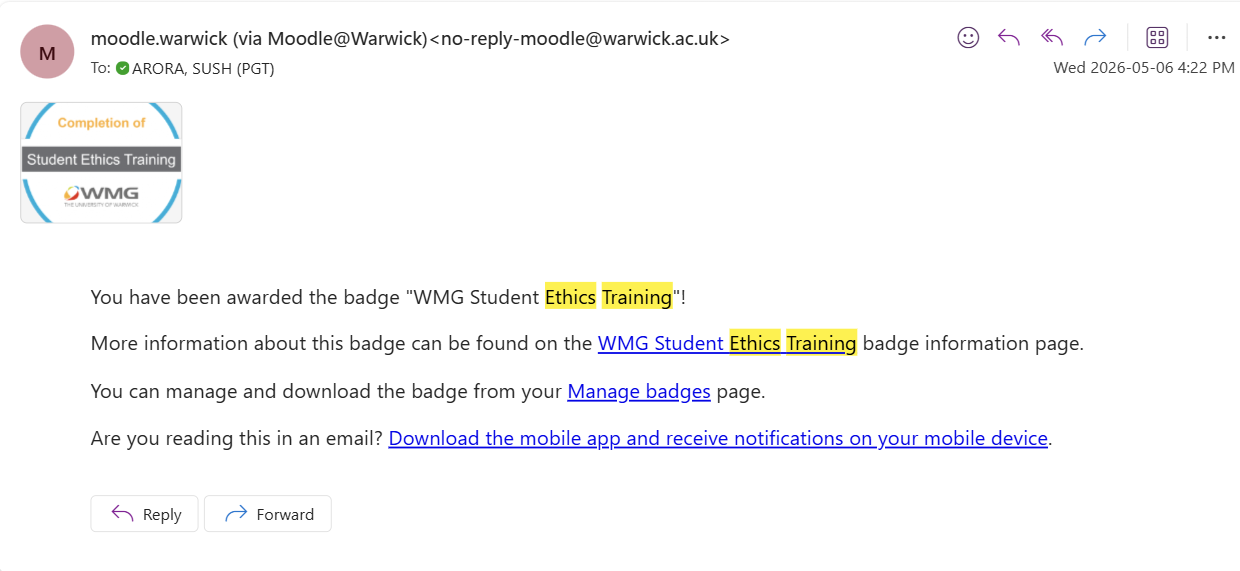
\includegraphics[
        width=0.96\textwidth,
        height=0.28\textheight,
        keepaspectratio
    ]{Images/Ethics_training.png}
    \caption{WMG Student Ethics Training completion evidence.}
    \label{fig:ethics-training}
\end{figure}

\section{Information Security Smart}
\label{sec:app-information-security}

The Information Security Smart course was completed to support appropriate handling of research data, code and computing resources. Figure~\ref{fig:information-security-smart} shows the completion evidence.

\begin{figure}[H]
    \centering
    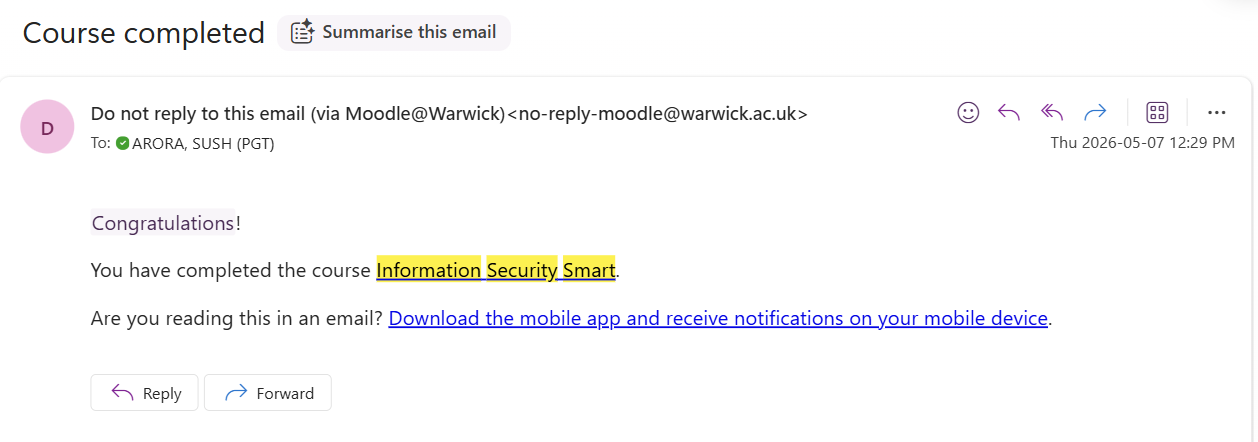
\includegraphics[
        width=0.96\textwidth,
        height=0.28\textheight,
        keepaspectratio
    ]{Images/Information_security_smart.png}
    \caption{Information Security Smart course completion evidence.}
    \label{fig:information-security-smart}
\end{figure}

\clearpage
\section{Responsible Research Practice}
\label{sec:app-responsible-research}

The Responsible Research Practice course was completed as part of the research training supporting this dissertation. Figure~\ref{fig:responsible-research-practice} reproduces the completion evidence.

\begin{figure}[H]
    \centering
    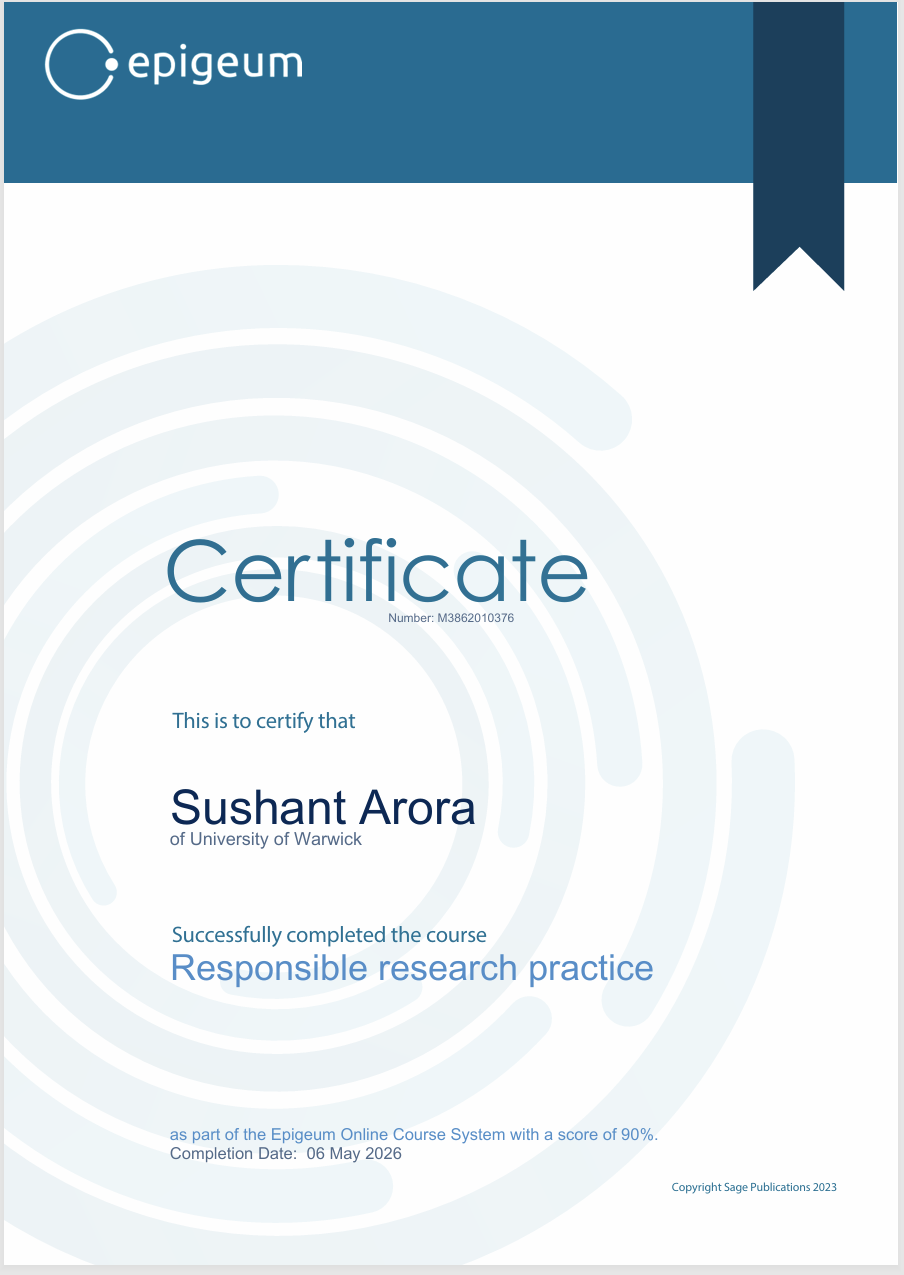
\includegraphics[
        width=0.78\textwidth,
        height=0.68\textheight,
        keepaspectratio
    ]{Images/Responsible_research_practice.png}
    \caption{Responsible Research Practice completion evidence.}
    \label{fig:responsible-research-practice}
\end{figure}

\clearpage
\section{Irresponsible Research Practice}
\label{sec:app-irresponsible-research}

The Irresponsible Research Practice course was also completed as part of the research training supporting this dissertation. Figure~\ref{fig:irresponsible-research-practice} reproduces the completion evidence.

\begin{figure}[H]
    \centering
    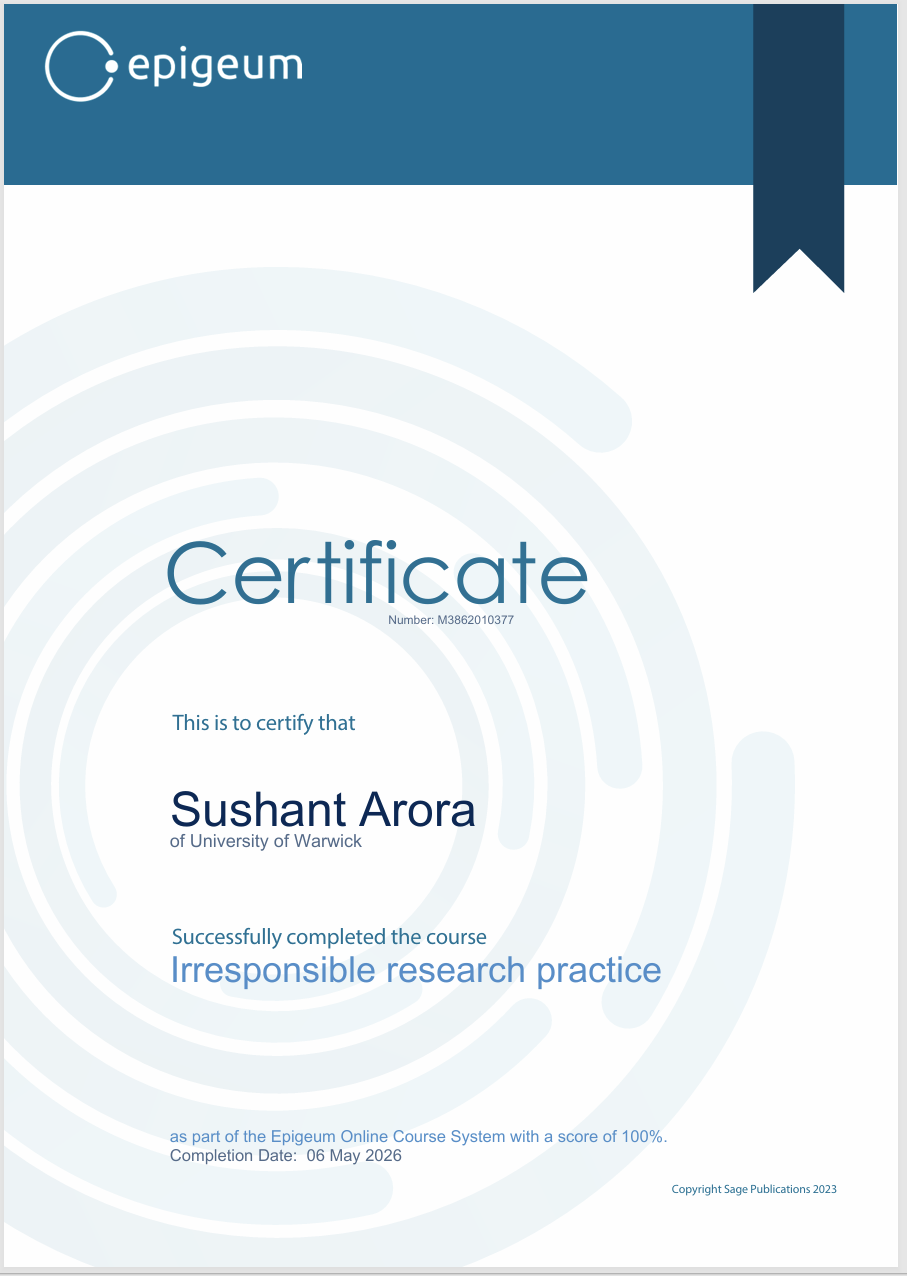
\includegraphics[
        width=0.78\textwidth,
        height=0.68\textheight,
        keepaspectratio
    ]{Images/Irresponsible_research_practice.png}
    \caption{Irresponsible Research Practice completion evidence.}
    \label{fig:irresponsible-research-practice}
\end{figure}


\chapter{Generative AI Declaration}
\label{app:generative-ai}

\section{Statement of Disclosure}
\label{sec:app-generative-ai-disclosure}

Generative Artificial Intelligence (GenAI) tools were used as supportive tools during the planning, development and preparation of this dissertation. Their use did not replace independent academic judgement, validation of experimental outputs or responsibility for the submitted work.

GenAI was used to generate boilerplate code and generic implementation patterns. This material was not adopted unchanged: it was reviewed, tested and modified for the specific data structures, model pipelines, evaluation logic and reproducibility requirements of the project. GenAI was also used for idea refinement and as a planning aid when developing the experimental execution strategy. This included considering experiment ordering, parallel execution, checkpointing and other practical choices intended to make efficient use of the available GPU hours.

Where GenAI-generated suggestions concerned code or experimental procedures, they were incorporated only after review and validation within the project workflow. GenAI outputs were not treated as experimental evidence and did not substitute for measured model outputs. The methodological decisions, verification of results, interpretation of findings and final submitted content remain the author's responsibility.

%
% Image files are expected to exist in the Images/ folder exactly as named below.

\chapter{Ethics and Security Documentation}
\label{app:ethics-security}

This appendix records the ethics, research-practice and information-security documentation supporting the study. The experimental work was conducted on research models and benchmark identity-document imagery rather than against live identity-verification services. The adversarial methods were used to evaluate the robustness of detection and localisation outputs within the defined research setting, not to demonstrate an operational verification bypass. The relevant University ethics confirmation and required training evidence are reproduced below.

\section{Ethics Approval}
\label{sec:app-ethics-approval}

The project was submitted through the University ethics process. Figure~\ref{fig:ethics-approval} reproduces the ethics approval or confirmation issued for the study.

\begin{figure}[H]
    \centering
    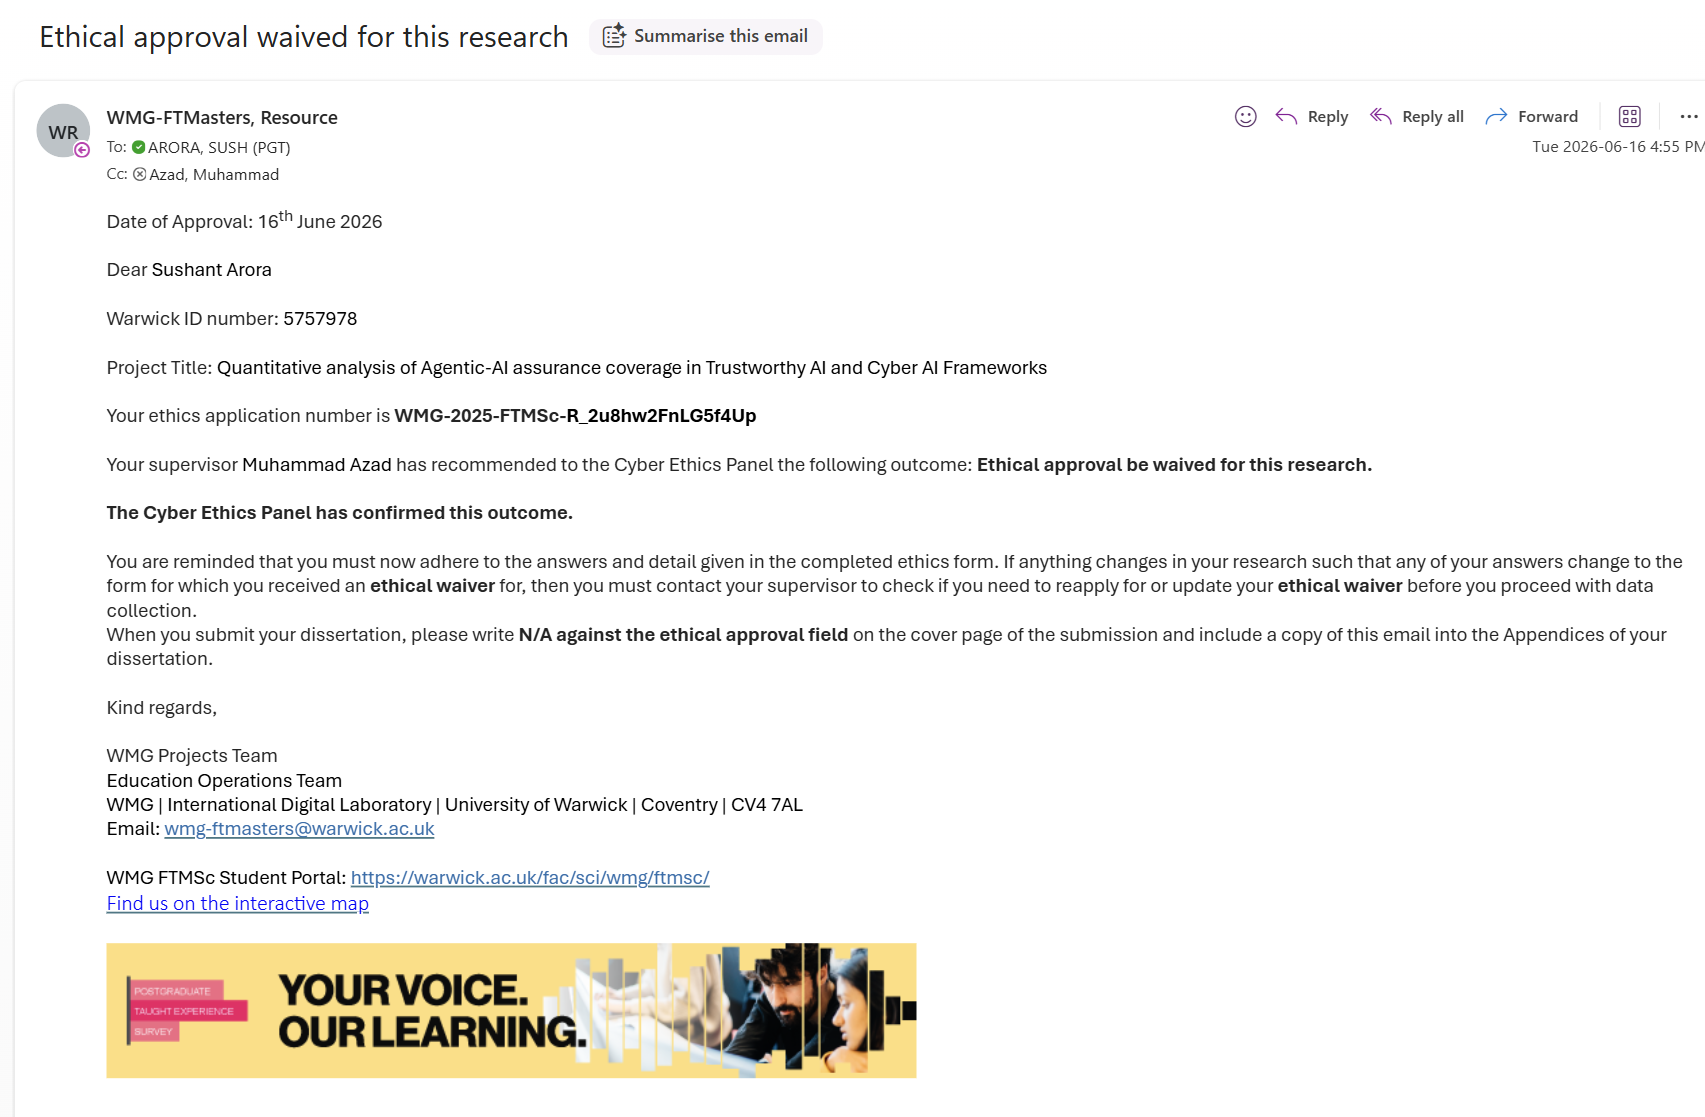
\includegraphics[
        width=0.95\textwidth,
        height=0.72\textheight,
        keepaspectratio
    ]{Images/Ethical_approval.png}
    \caption{Ethics approval or confirmation for the research project.}
    \label{fig:ethics-approval}
\end{figure}

\clearpage
\section{WMG Student Ethics Training}
\label{sec:app-ethics-training}

The WMG Student Ethics Training was completed as part of the research-governance requirements for the project. Figure~\ref{fig:ethics-training} shows the completion evidence.

\begin{figure}[H]
    \centering
    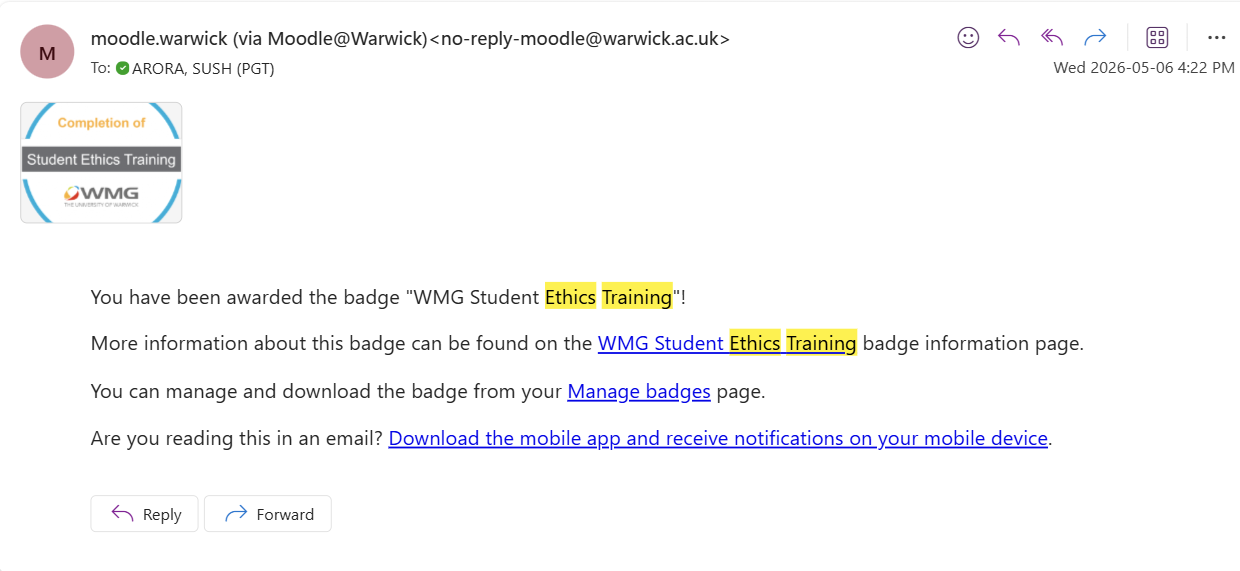
\includegraphics[
        width=0.96\textwidth,
        height=0.28\textheight,
        keepaspectratio
    ]{Images/Ethics_training.png}
    \caption{WMG Student Ethics Training completion evidence.}
    \label{fig:ethics-training}
\end{figure}

\section{Information Security Smart}
\label{sec:app-information-security}

The Information Security Smart course was completed to support appropriate handling of research data, code and computing resources. Figure~\ref{fig:information-security-smart} shows the completion evidence.

\begin{figure}[H]
    \centering
    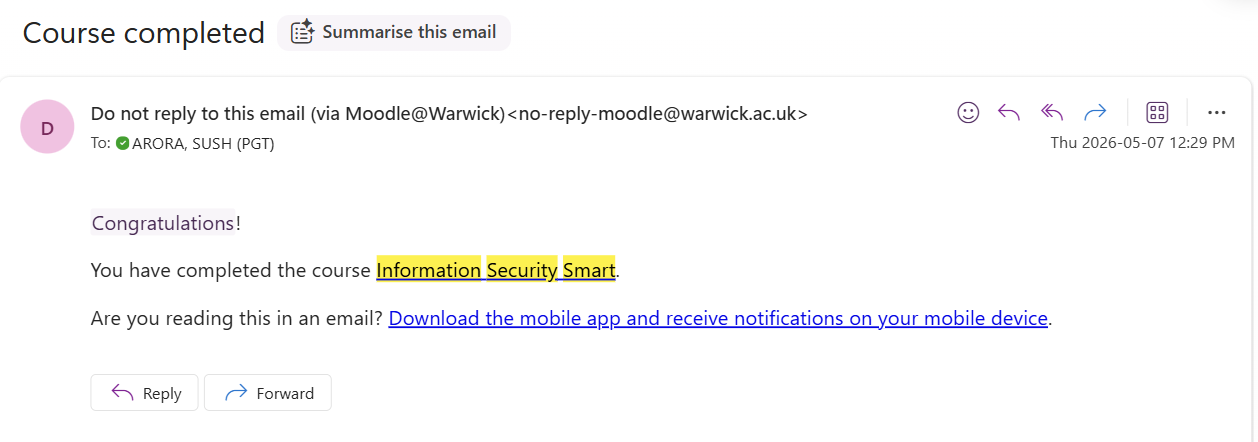
\includegraphics[
        width=0.96\textwidth,
        height=0.28\textheight,
        keepaspectratio
    ]{Images/Information_security_smart.png}
    \caption{Information Security Smart course completion evidence.}
    \label{fig:information-security-smart}
\end{figure}

\clearpage
\section{Responsible Research Practice}
\label{sec:app-responsible-research}

The Responsible Research Practice course was completed as part of the research training supporting this dissertation. Figure~\ref{fig:responsible-research-practice} reproduces the completion evidence.

\begin{figure}[H]
    \centering
    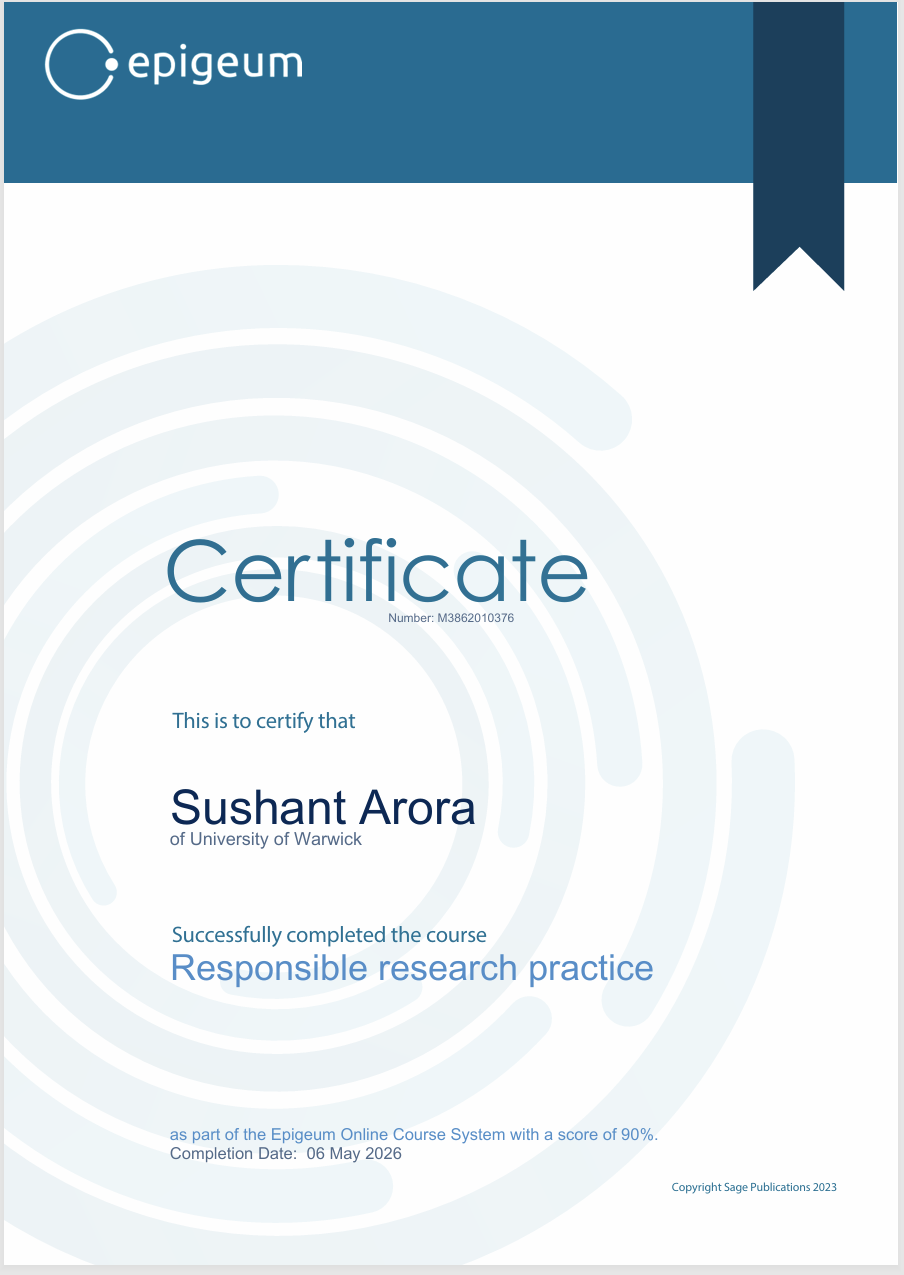
\includegraphics[
        width=0.78\textwidth,
        height=0.68\textheight,
        keepaspectratio
    ]{Images/Responsible_research_practice.png}
    \caption{Responsible Research Practice completion evidence.}
    \label{fig:responsible-research-practice}
\end{figure}

\clearpage
\section{Irresponsible Research Practice}
\label{sec:app-irresponsible-research}

The Irresponsible Research Practice course was also completed as part of the research training supporting this dissertation. Figure~\ref{fig:irresponsible-research-practice} reproduces the completion evidence.

\begin{figure}[H]
    \centering
    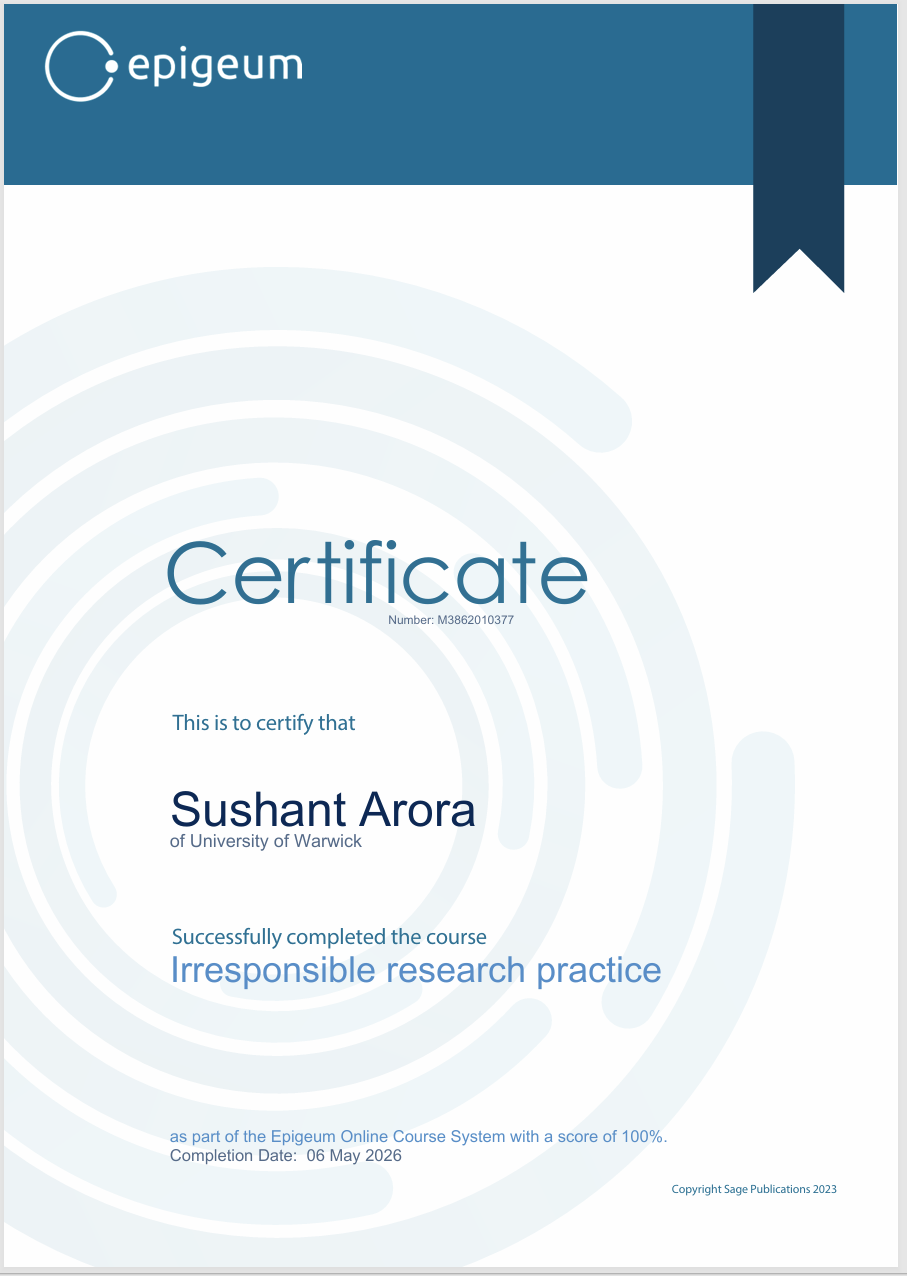
\includegraphics[
        width=0.78\textwidth,
        height=0.68\textheight,
        keepaspectratio
    ]{Images/Irresponsible_research_practice.png}
    \caption{Irresponsible Research Practice completion evidence.}
    \label{fig:irresponsible-research-practice}
\end{figure}


\chapter{Generative AI Declaration}
\label{app:generative-ai}

\section{Statement of Disclosure}
\label{sec:app-generative-ai-disclosure}

Generative Artificial Intelligence (GenAI) tools were used as supportive tools during the planning, development and preparation of this dissertation. Their use did not replace independent academic judgement, validation of experimental outputs or responsibility for the submitted work.

GenAI was used to generate boilerplate code and generic implementation patterns. This material was not adopted unchanged: it was reviewed, tested and modified for the specific data structures, model pipelines, evaluation logic and reproducibility requirements of the project. GenAI was also used for idea refinement and as a planning aid when developing the experimental execution strategy. This included considering experiment ordering, parallel execution, checkpointing and other practical choices intended to make efficient use of the available GPU hours.

Where GenAI-generated suggestions concerned code or experimental procedures, they were incorporated only after review and validation within the project workflow. GenAI outputs were not treated as experimental evidence and did not substitute for measured model outputs. The methodological decisions, verification of results, interpretation of findings and final submitted content remain the author's responsibility.

%
% Image files are expected to exist in the Images/ folder exactly as named below.

\chapter{Ethics and Security Documentation}
\label{app:ethics-security}

This appendix records the ethics, research-practice and information-security documentation supporting the study. The experimental work was conducted on research models and benchmark identity-document imagery rather than against live identity-verification services. The adversarial methods were used to evaluate the robustness of detection and localisation outputs within the defined research setting, not to demonstrate an operational verification bypass. The relevant University ethics confirmation and required training evidence are reproduced below.

\section{Ethics Approval}
\label{sec:app-ethics-approval}

The project was submitted through the University ethics process. Figure~\ref{fig:ethics-approval} reproduces the ethics approval or confirmation issued for the study.

\begin{figure}[H]
    \centering
    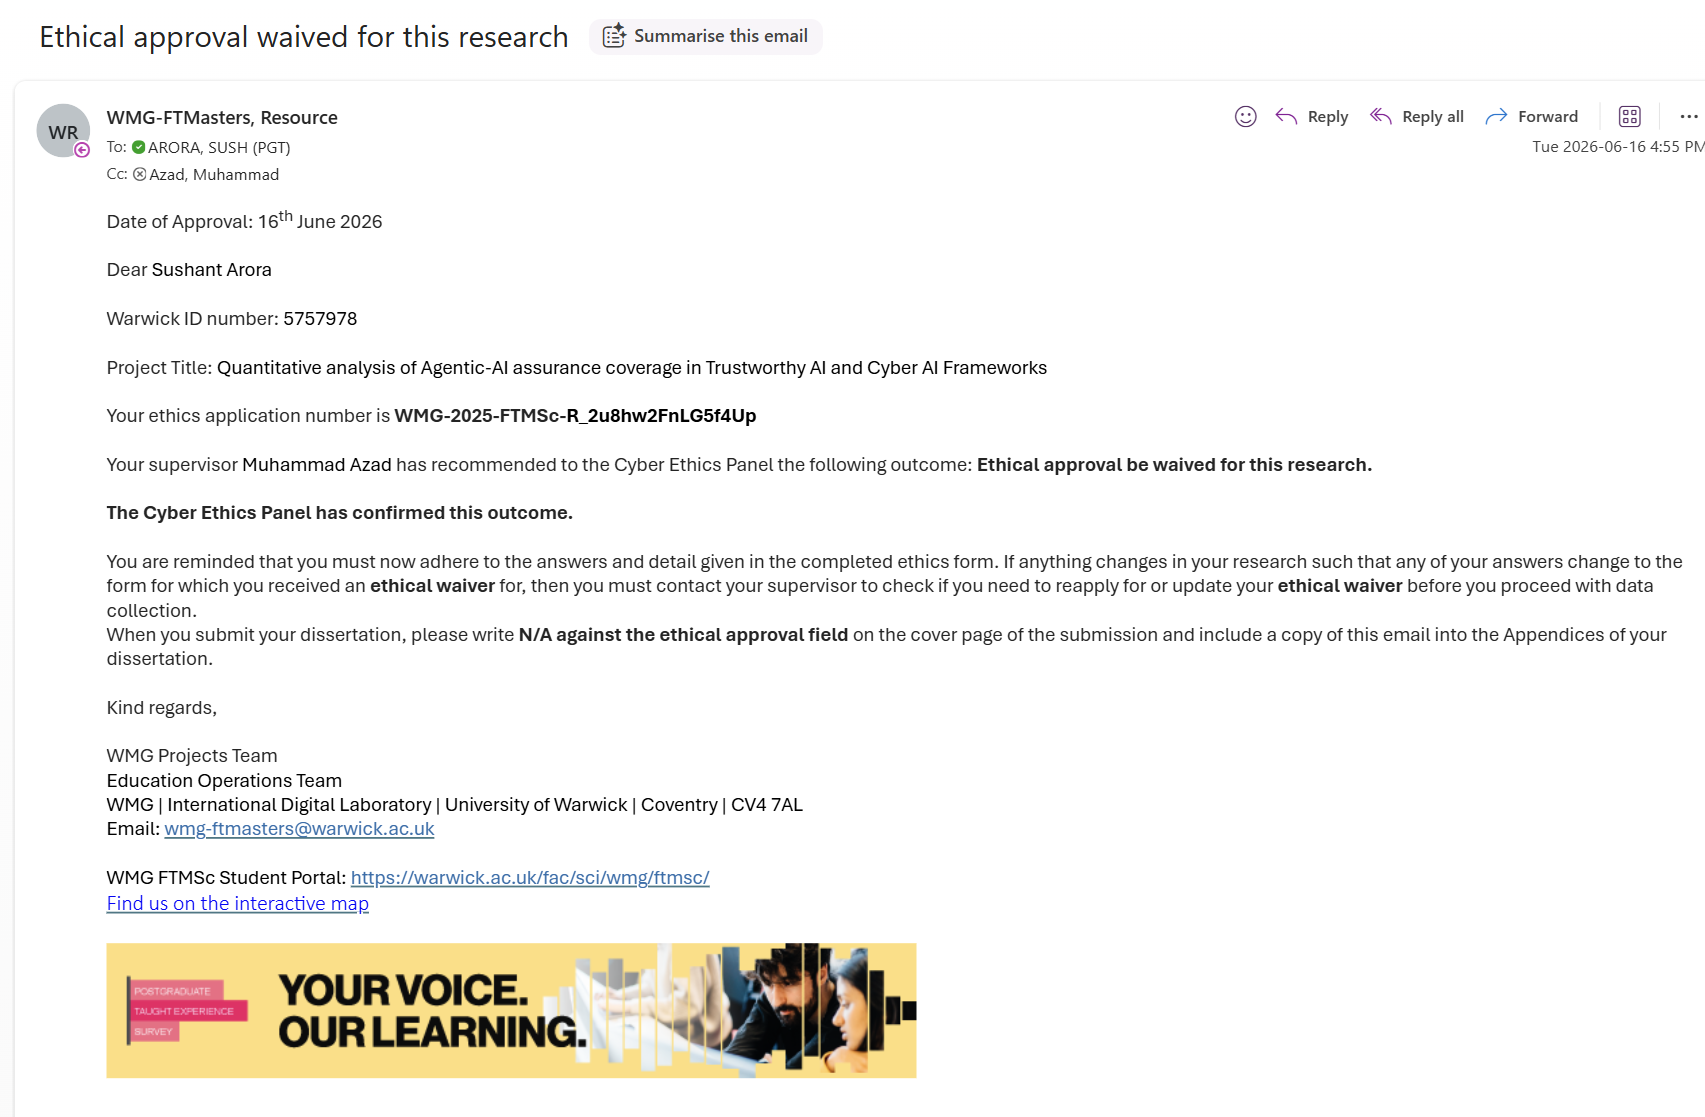
\includegraphics[
        width=0.95\textwidth,
        height=0.72\textheight,
        keepaspectratio
    ]{Images/Ethical_approval.png}
    \caption{Ethics approval or confirmation for the research project.}
    \label{fig:ethics-approval}
\end{figure}

\clearpage
\section{WMG Student Ethics Training}
\label{sec:app-ethics-training}

The WMG Student Ethics Training was completed as part of the research-governance requirements for the project. Figure~\ref{fig:ethics-training} shows the completion evidence.

\begin{figure}[H]
    \centering
    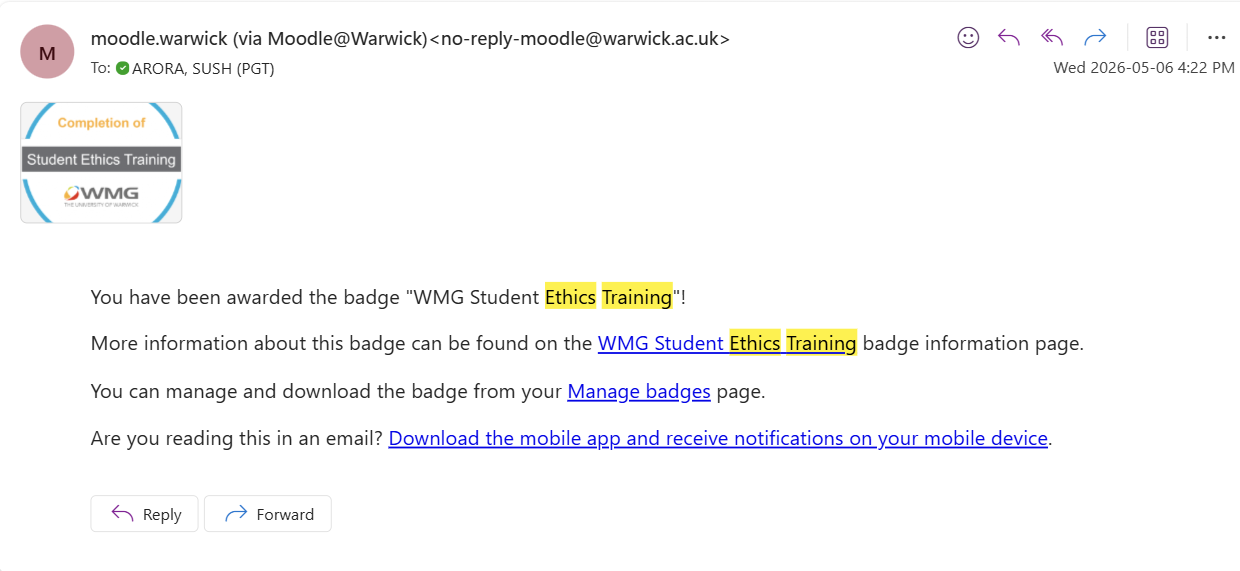
\includegraphics[
        width=0.96\textwidth,
        height=0.28\textheight,
        keepaspectratio
    ]{Images/Ethics_training.png}
    \caption{WMG Student Ethics Training completion evidence.}
    \label{fig:ethics-training}
\end{figure}

\section{Information Security Smart}
\label{sec:app-information-security}

The Information Security Smart course was completed to support appropriate handling of research data, code and computing resources. Figure~\ref{fig:information-security-smart} shows the completion evidence.

\begin{figure}[H]
    \centering
    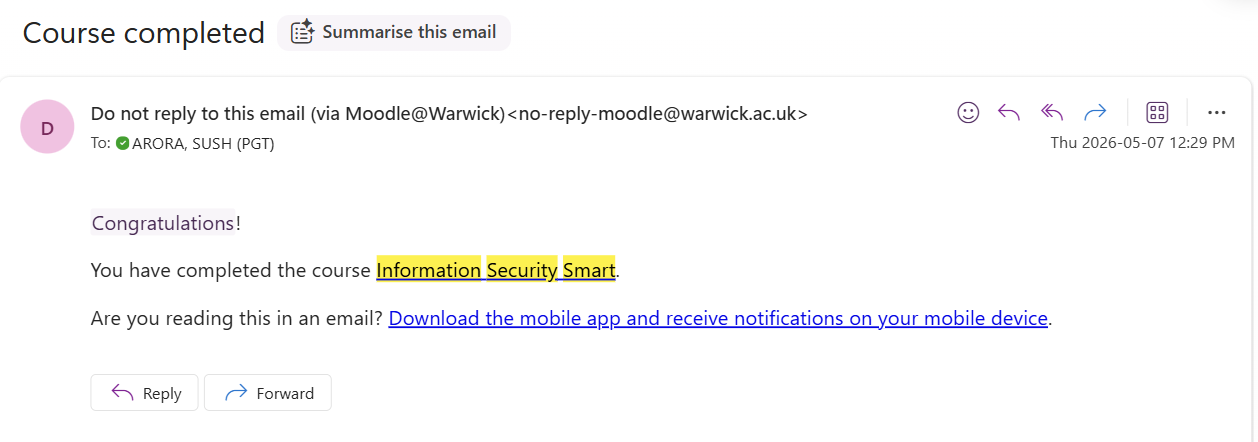
\includegraphics[
        width=0.96\textwidth,
        height=0.28\textheight,
        keepaspectratio
    ]{Images/Information_security_smart.png}
    \caption{Information Security Smart course completion evidence.}
    \label{fig:information-security-smart}
\end{figure}

\clearpage
\section{Responsible Research Practice}
\label{sec:app-responsible-research}

The Responsible Research Practice course was completed as part of the research training supporting this dissertation. Figure~\ref{fig:responsible-research-practice} reproduces the completion evidence.

\begin{figure}[H]
    \centering
    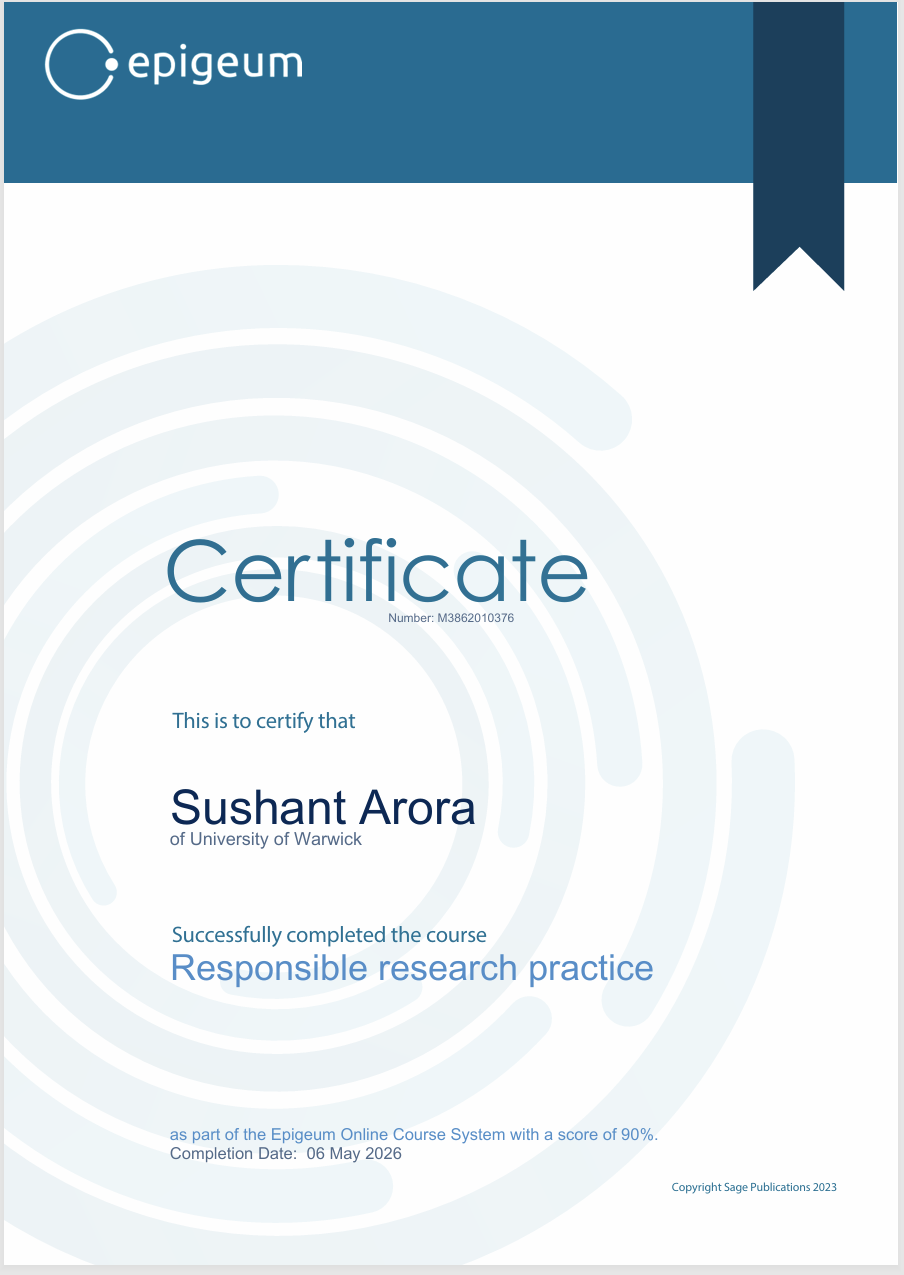
\includegraphics[
        width=0.78\textwidth,
        height=0.68\textheight,
        keepaspectratio
    ]{Images/Responsible_research_practice.png}
    \caption{Responsible Research Practice completion evidence.}
    \label{fig:responsible-research-practice}
\end{figure}

\clearpage
\section{Irresponsible Research Practice}
\label{sec:app-irresponsible-research}

The Irresponsible Research Practice course was also completed as part of the research training supporting this dissertation. Figure~\ref{fig:irresponsible-research-practice} reproduces the completion evidence.

\begin{figure}[H]
    \centering
    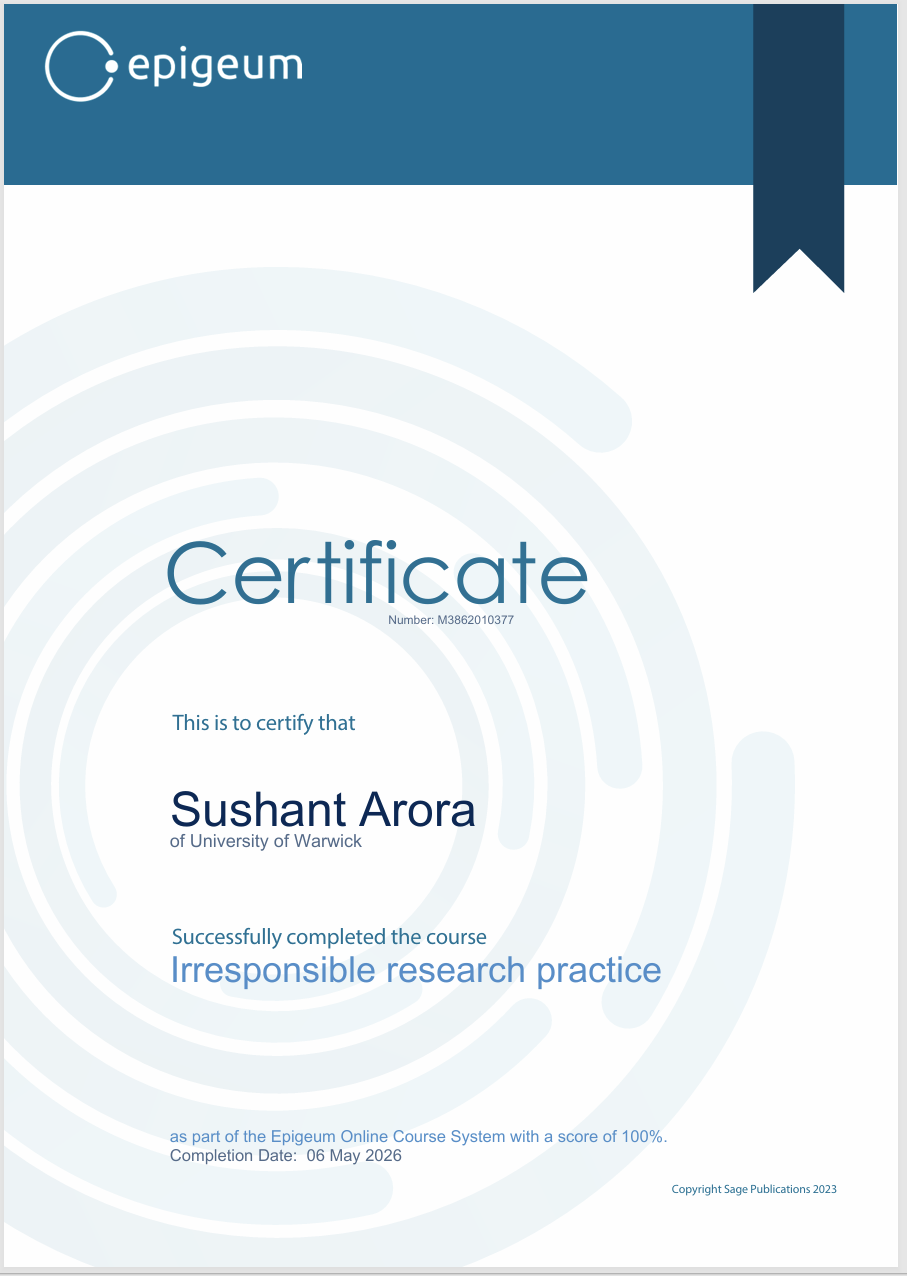
\includegraphics[
        width=0.78\textwidth,
        height=0.68\textheight,
        keepaspectratio
    ]{Images/Irresponsible_research_practice.png}
    \caption{Irresponsible Research Practice completion evidence.}
    \label{fig:irresponsible-research-practice}
\end{figure}


\chapter{Generative AI Declaration}
\label{app:generative-ai}

\section{Statement of Disclosure}
\label{sec:app-generative-ai-disclosure}

Generative Artificial Intelligence (GenAI) tools were used as supportive tools during the planning, development and preparation of this dissertation. Their use did not replace independent academic judgement, validation of experimental outputs or responsibility for the submitted work.

GenAI was used to generate boilerplate code and generic implementation patterns. This material was not adopted unchanged: it was reviewed, tested and modified for the specific data structures, model pipelines, evaluation logic and reproducibility requirements of the project. GenAI was also used for idea refinement and as a planning aid when developing the experimental execution strategy. This included considering experiment ordering, parallel execution, checkpointing and other practical choices intended to make efficient use of the available GPU hours.

Where GenAI-generated suggestions concerned code or experimental procedures, they were incorporated only after review and validation within the project workflow. GenAI outputs were not treated as experimental evidence and did not substitute for measured model outputs. The methodological decisions, verification of results, interpretation of findings and final submitted content remain the author's responsibility.
